\documentclass[14pt,fleqn,a4paper]{scrartcl}
\binoppenalty=1000
\relpenalty=1000
\usepackage[utf8]{inputenc}
\usepackage[unicode, pdftex,pdfborder=0 0 0,colorlinks, linkcolor=black]{hyperref}
\usepackage[english,russian]{babel}
\usepackage{indentfirst}
\usepackage{booktabs}
\usepackage{misccorr}
\usepackage{graphicx}
\usepackage{multirow}
\usepackage{tikz}
\usepackage{amsmath}
\usepackage{wrapfig}
\usepackage{longtable}
\usepackage{algorithm2e}
\usepackage{mathtools}
\begin{document}

\begin{center}
МОСКОВСКИЙ ГОСУДАРСТВЕННЫЙ УНИВЕРСИТЕТ \\ имени М. В. ЛОМОНОСОВА\\ Механико-математический факультет
\end{center}
\begin{figure}[htbp]
\centering
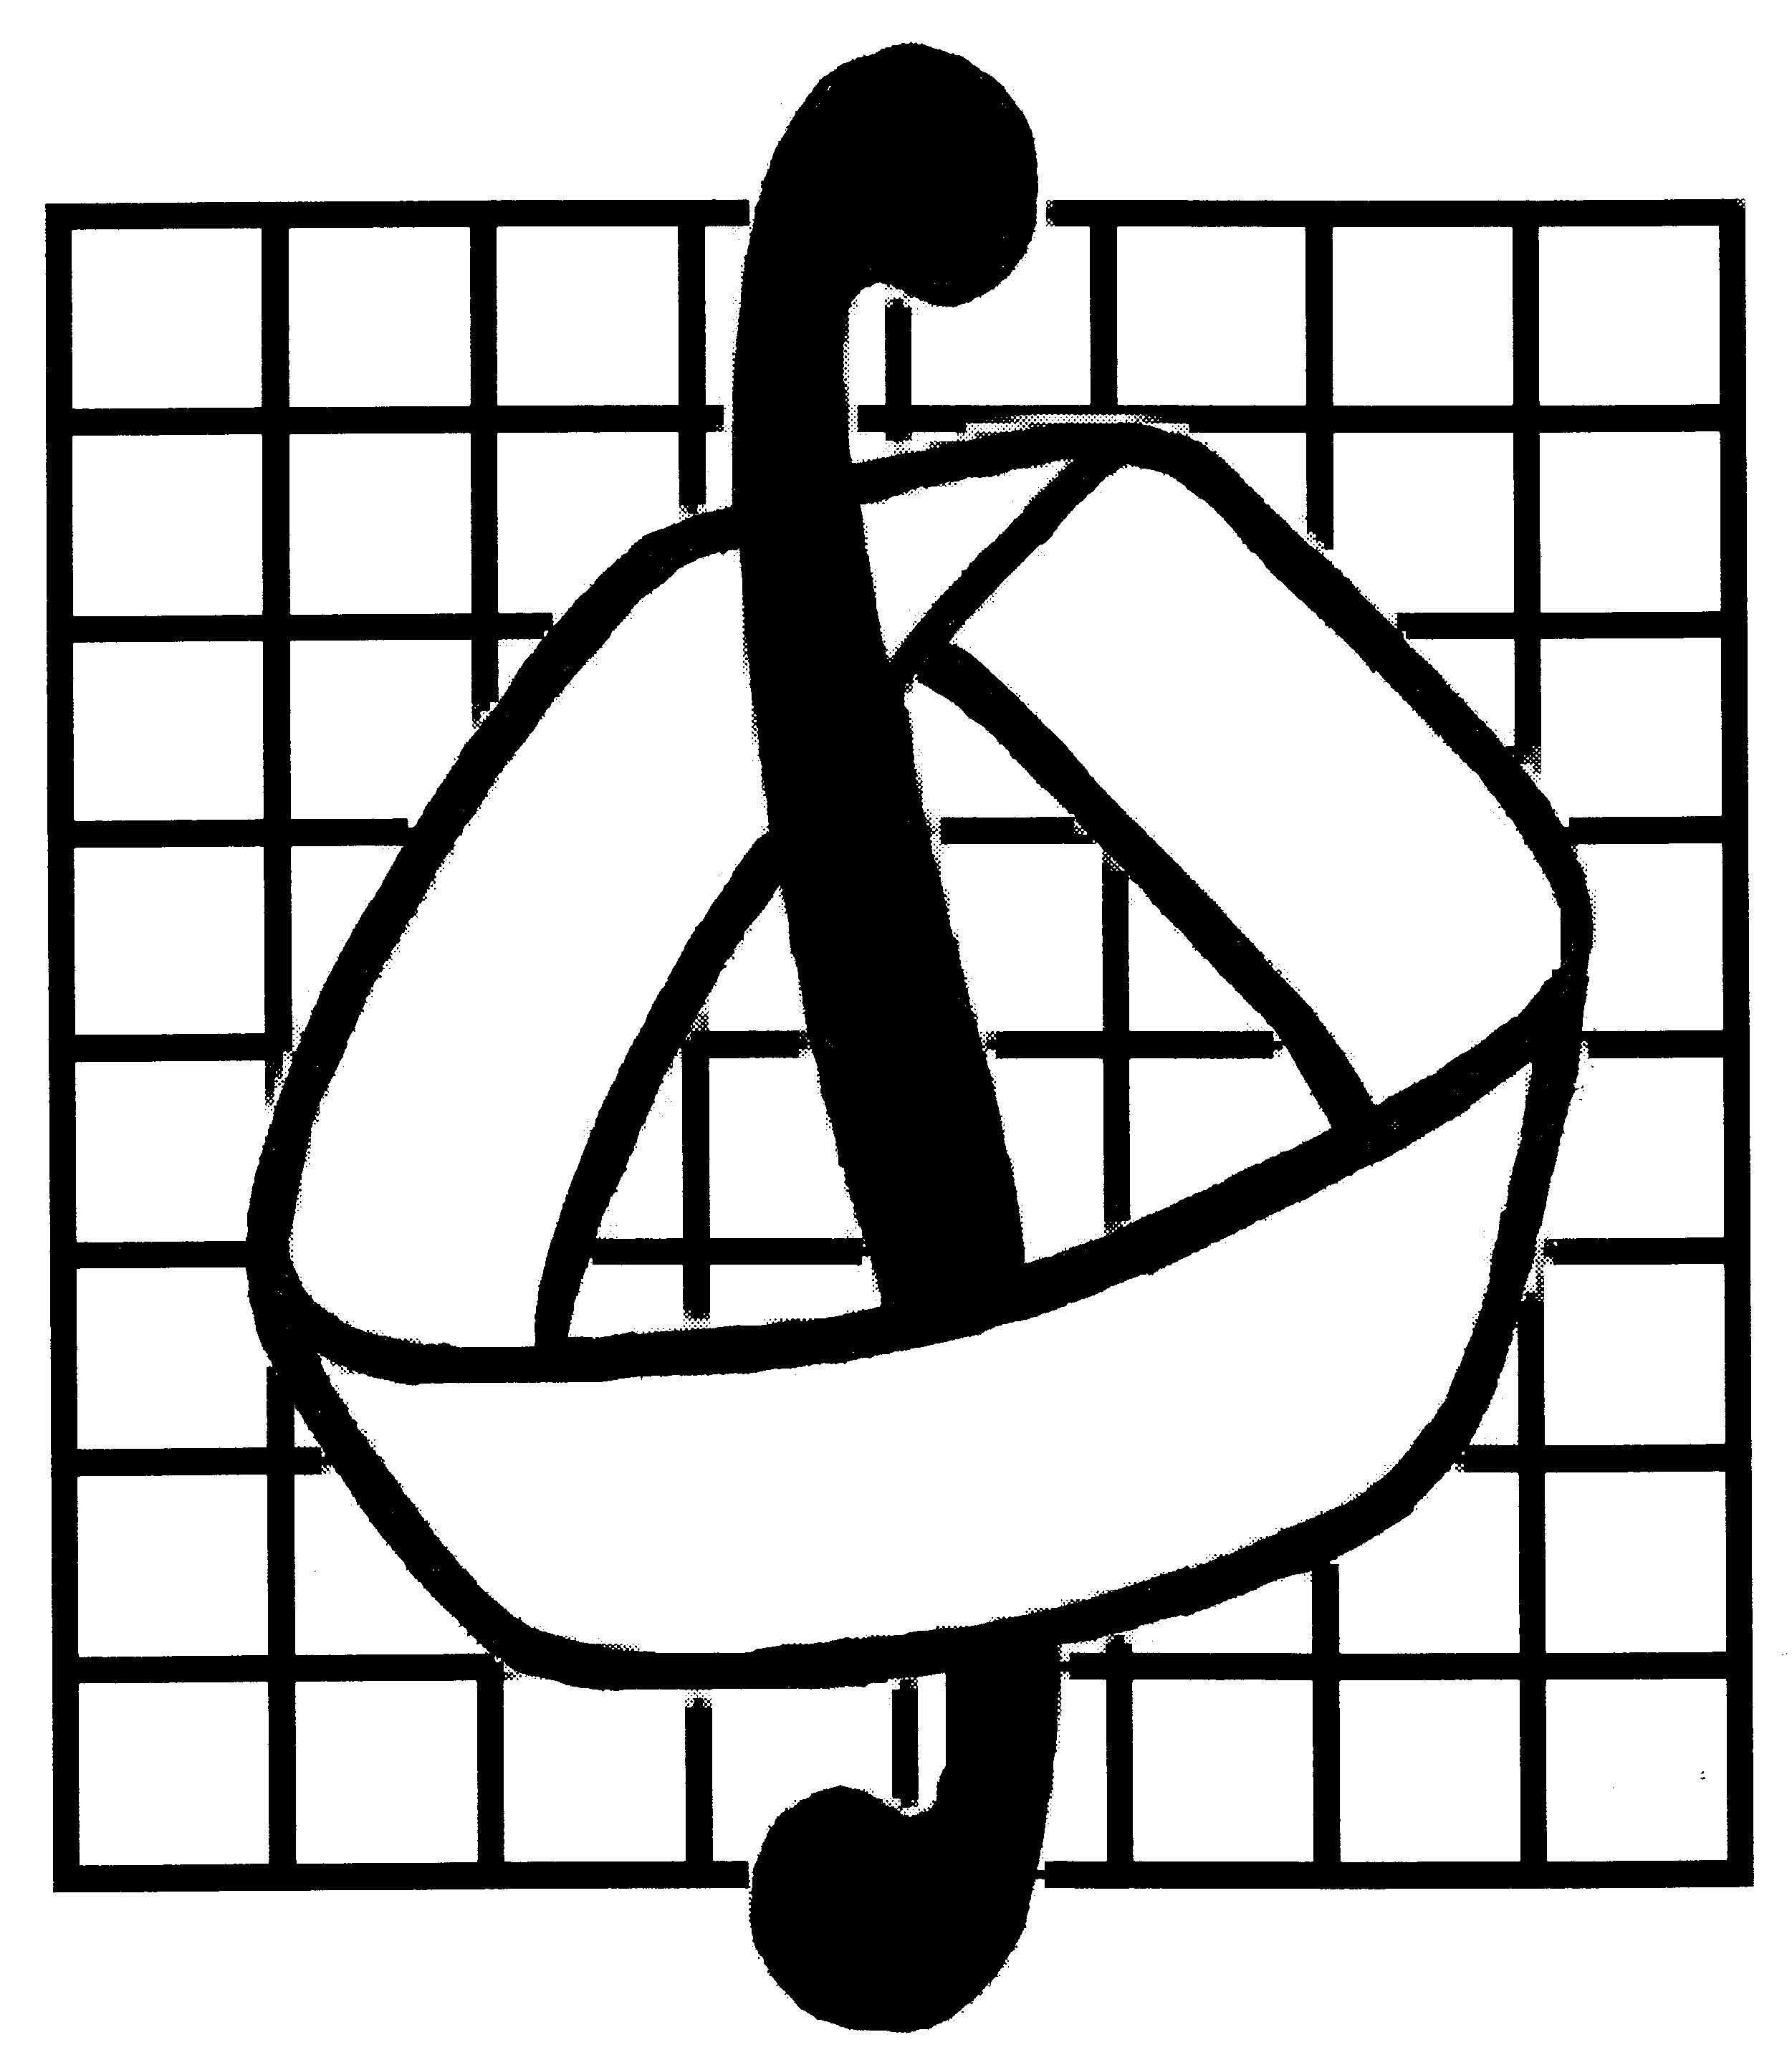
\includegraphics[width=0.3\textwidth]{36cacac6.png}
\end{figure}
\begin{center}
\textbf{\large{\textit{Курсовая работа.}}}
\end{center} 
\textbf{\large{\textit{Аппроксимация многогранника по набору пространственных отрезков. Построение многогранника по набору полупространств.}}} \\
\begin{flushright} {Научный руководитель: Валединский В.Д.\\ }\end{flushright}
\begin{flushright} {Студент: Ковальков М.Н.\\ }\end{flushright}
\newpage 
\tableofcontents
\newpage
\section{Введение}
\subsection{Происхождение задачи.}
Данная работа возникла из задачи оценки качества огранки драгоценных камней. 
\section{Задача аппроксимации многогранника по набору пространственных отрезков.}
\subsection{Постановка задачи.}
Имеется многогранник и набор целевых ребер. Предполагается, что многогранник построен неточно, а целевые ребра-точны. Требуется изменить многогранник так, чтобы он наилчшим образом соответствовал целевым ребрам.
\begin{center}
\begin{tabular}{cc}

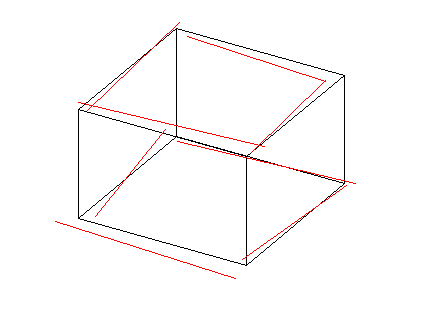
\includegraphics[width=0.5\textwidth]{input.png} &
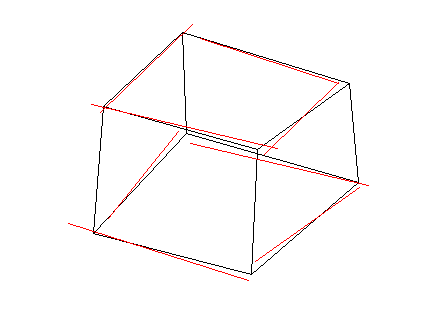
\includegraphics[width=0.5\textwidth]{out.png} \\
Исходный многогранник& Измененный многогранник \\
\\
\end{tabular}
\end{center}
\subsection{Математическая формализация задачи. Построение минимализируемого функционала}
Имеется многогранник $M$, заданный наборами своих граней, ребер и вершин.
$$
\begin{cases}
p_{i}=(x_{i},y_{i},z_{i})- &\text{Координаты вершин многогранника, } i=\overline{1,n_{1}} \\ 
e_{j}=(a_{j,1}, a_{j,2})- & \begin{array}[c]{ll}%
\text{Номера вершин, которые являются}
\\
\text{концами ребра } e_{j} \text{, } j=\overline{1,n_{2}}
\end{array}\\ 
f_{k}=[b_{k,1}, \ldots, b_{k,m_{k}}] - & \text{Номера ребер, входящих в грань } f_{k} \text{, } k=\overline{1,n_{3}} \\
\end{cases}
$$ 
Имеется список целевых ребер, которые считаются точными и которые поставлены в соответствие исходным ребрам многогранника.
$$
\widetilde{e_{i}}=
\begin{cases}
(a_{i,x},a_{i,y},a_{i,z}),(b_{i,x},b_{i,y},b_{i,z})-
\text{координаты двух концов данного целевого ребра. } \\ 
ind_{i}-
\text{номер исходного ребра,
которому соответствует i-е целевое ребро. } 
\end{cases}
$$
\par
Если в списке целевых ребер нет элемента для текущего ребра, то считаем, что оно является целевым само для себя. Однако вес, с которым оно входит в функционал будет равен $\omega_{i}=0.1$, в то время, как для полноценного целевого ребра $\omega_{i}=1$. После расширения списка целевых ребер указанным способом, будем считать, что $\widetilde{e_{i}}$-целевое ребро, соответствующее исходному ребру $e_{i}$ многогранника $M$.\par
Сделаем ребра многогранника "подвижными", для этого введём переменные $\tilde p_{i,1}=(\tilde x_{i,1},\tilde y_{i,1},\tilde z_{i,1}),\tilde p_{i,1}=(\tilde x_{i,2},\tilde y_{i,2},\tilde z_{i,2}) $, соответствующие концам "подвижных" ребер. Мы хотим найти такую конфигурацию, чтобы эти ребра были наименее удалены от соответствующим им целевых. Для этого мы должны доставить минимум следующего функционала:
$$\sum_{i=1}^{n_{2}}\omega_{i}(\rho^{2}(\tilde p_{i,1},\widetilde{e_{i}})+\rho^{2}(\tilde p_{i,2},\widetilde{e_{i}}))\rightarrow \min , \text{ где}$$ 
$\rho(\tilde p_{i,j},\widetilde{e_{i}})$-расстояние между концами "движимого" ребра и прямой, заданной соответствующим целевым ребром. 
\begin{figure}[htbp]
\centering
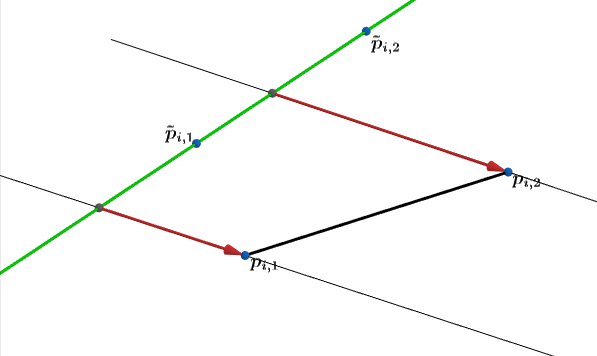
\includegraphics[width=0.7\textwidth]{distancce.png}
\end{figure}
\subsection{Вычисление расстояния от точки до прямой.}

Для вычисления расстояние воспользуемся формулой вычисления проекции вектора $\overrightarrow{a}$ на вектор $\overrightarrow{b}$: \\
\begin{wrapfigure}[8]{r}{0.15\linewidth} 
\begin{tikzpicture}
\coordinate [label=1:$L_{1}$] (A) at (0,0);
\coordinate [label=2:$L_{2}$] (B) at (1,3);
\coordinate [label=3:$P$](C) at (1.8,1.4);
\coordinate [label=4:$P'$](D) at (0.6,1.8);
\draw [->,black] (A) -- (B);
\draw [->,black] (A) -- (C);
\draw [red] (C) -- (D);
\draw [->,black] (A) -- (D);
\end{tikzpicture}
\end{wrapfigure}
$$pr_{\overrightarrow{L_{1}L_{2}}} \overrightarrow{L_{1}P}=\frac{( \overrightarrow{L_{1}P}, \overrightarrow{L_{1}L_{2}})}{ (\overrightarrow{L_{1}L_{2}}, \overrightarrow{L_{1}L_{2}})} \overrightarrow{L_{1}L_{2}},\text{ где}$$ (*,*) -- стандартное скалярное произведение:
$$( \overrightarrow{a}, \overrightarrow{b})=a_{x}b_{x}+a_{y}b_{y}+a_{z}b_{z}$$
Далее пользуемся теоремой Пифагора для вычисления расстояния:

$$\rho^{2}(P,L_1L_2)=|\overrightarrow{L_{1}P}|^{2}-|pr_{\overrightarrow{L_{1}L_{2}}} \overrightarrow{L_{1}P}|^{2}=\frac{(\overrightarrow{L_{1}P},\overrightarrow{L_{1}P})(\overrightarrow{L_{1}L_{2}},\overrightarrow{L_{1}L_{2}})-(\overrightarrow{L_{1}P},\overrightarrow{L_{1}L_{2}})(\overrightarrow{L_{1}P},\overrightarrow{L_{1}L_{2}})}{(\overrightarrow{L_{1}L_{2}},\overrightarrow{L_{1}L_{2}})}$$

\subsection{Доказательство выпуклости функционала.}
Для корректности применения метода внутренней точки требуется выпуклость минимализируемого функционала. Докажем, что рассматриваемый нами функционал-выпуклый. 
Рассмотрим одно слагаемое суммы, образующей наш функционал:
$$
F=(x-a_{x})^{2}+(y-a_{y})^{2}+(z-a_{z})^{2}-\frac{((x-a_{x})(b_{x}-a_{x})+(x-a_{y})(b_{y}-a_{y})+(x-a_{z})(b_{z}-a_{z}))^{2}}{(b_{x}-a_{x})^2+(b_{y}-a_{y})^2+(b_{z}-a_{z})^2}
$$
Введем обозначения: $c_{1}:=(b_{x}-a_{x}),c_{2}:=(b_{y}-a_{y}),c_{3}:=(b_{z}-a_{z}),c:=c_{1}^{2}+c_{2}^{2}+c_{3}^{2}$.\\ И запишем матрицу вторых частных производных $F$:
$$
\begin{pmatrix}
\frac{\partial^{2}F}{\partial x^{2}} & \frac{\partial^{2}F}{\partial x \partial y} & \frac{\partial^{2}F}{\partial x \partial z} \\
\frac{\partial^{2}F}{\partial y \partial x} & \frac{\partial^{2}F}{\partial y^{2}} & \frac{\partial^{2}F}{\partial y \partial z} \\
\frac{\partial^{2}F}{\partial z\partial x} & \frac{\partial^{2}F}{\partial z \partial y} & \frac{\partial^{2}F}{\partial z^{2}} \\
\end{pmatrix}
=
\begin{pmatrix}
2(1-\frac{c_{1}^{2}}{c}) & -\frac{c_{1}c_{2}}{c} & -\frac{c_{1}c_{3}}{c}\\
-\frac{c_{1}c_{2}}{c}& 2(1-\frac{c_{2}^{2}}{c}) & -\frac{c_{2}c_{3}}{c}\\
-\frac{c_{1}c_{3}}{c}& -\frac{c_{2}c_{3}}{c} & 2(1-\frac{c_{3}^{2}}{c}) \\
\end{pmatrix}
$$
Проверим матрицу на неотрицательную определенность с помощью Критерия Сильвестра. Для этого вычислим определители главных миноров.\\
1)$|\Delta_{1}|=2\frac{c_{2}^{2}+c_{3}^{2}}{c}\geq 0$\\
2)$|\Delta_{2}|
=
\begin{vmatrix}
2(1-\frac{c_{1}^{2}}{c}) & -\frac{c_{1}c_{2}}{c} \\
-\frac{c_{1}c_{2}}{c}& 2(1-\frac{c_{2}^{2}}{c}) \\
\end{vmatrix}=
4-4\frac{c_{1}^{2}+c_{2}^{2}}{c}+4\frac{c_{1}^{2}c_{2}^{2}}{c^{2}}-\frac{c_{1}^{2}c_{2}^{2}}{c^{2}}=4\frac{c_{3}^{2}}{c}+3\frac{c_{1}^{2}c_{2}^{2}}{c^{2}}\geq 0
$\\
3) $|\Delta_{3}|=
\begin{vmatrix}
2(1-\frac{c_{1}^{2}}{c}) & -\frac{c_{1}c_{2}}{c} & -\frac{c_{1}c_{3}}{c}\\
-\frac{c_{1}c_{2}}{c}& 2(1-\frac{c_{2}^{2}}{c}) & -\frac{c_{2}c_{3}}{c}\\
-\frac{c_{1}c_{3}}{c}& -\frac{c_{2}c_{3}}{c} & 2(1-\frac{c_{3}^{2}}{c}) \\
\end{vmatrix}=
8(1-\frac{c_{1}^{2}}{c})(1-\frac{c_{2}^{2}}{c})(1-\frac{c_{3}^{2}}{c})-2\frac{c_{1}^{2}c_{2}^{2}c_{3}^{2}}{c^{3}}- \\ -
2\frac{c_{1}^{2}c_{3}^{2}}{c^{2}}(1-\frac{c_{2}^{2}}{c})-2\frac{c_{2}^{2}c_{3}^{2}}{c^{2}}(1-\frac{c_{1}^{2}}{c})
-\frac{c_{1}^{2}c_{2}^{2}}{c^{2}}(1-\frac{c_{3}^{2}}{c})= 8 - 4\frac{c_{1}^{2}c_{2}^{2}c_{3}^{2}}{c^{3}}+6(\frac{c_{1}^{2}c_{2}^{2}}{c^{2}}+\frac{c_{1}^{2}c_{3}^{2}}{c^{2}}+\frac{c_{2}^{2}c_{3}^{2}}{c^{2}})-8\frac{c_{1}^{2}+c_{2}^{2}+c_{3}^{2}}{c}= \\ =6(\frac{c_{1}^{2}c_{2}^{2}}{c^{2}}+\frac{c_{1}^{2}c_{3}^{2}}{c^{2}})+2(\frac{c_{2}^{2}c_{3}^{2}}{c^{2}})+4+\frac{c_{2}^{2}c_{3}^{2}}{c^{2}}(1-\frac{c_{1}^{2}}{c})=6(\frac{c_{1}^{2}c_{2}^{2}}{c^{2}}+\frac{c_{1}^{2}c_{3}^{2}}{c^{2}})+2(\frac{c_{2}^{2}c_{3}^{2}}{c^{2}})+4+\frac{c_{2}^{2}c_{3}^{2}}{c^{2}}(\frac{c_{2}^{2}+c_{3}^{2}}{c})\geq 0
$\\
Тем самым мы показали, что матрица вторых частных производных функции- неотрицательна, следовательно эта функция является выпуклой. Осталось вспомнить, что сумма выпуклых функций также является выпуклой (Прямое следствие определения через неравенство Йенсена).\par 
Таким образом, показана выпуклость задачи и, как следствие, корректность применения метода внутренней точки для её решения. 
\subsection{Условия, налагаемые на функционал.}
На функционал нужно наложить ряд ограничений, основным из которых является следующее: если исходные ребра лежали в одной грани, то и "подвижные" ребра должны лежать в одной грани. Иными словами:
$$
\forall k=\overline{1,n_{3}} \text{ } \exists \text{ плоскость } \pi_{k} : \forall j \in f_{k}, \overline{\tilde{p}_{j,1},\tilde{p}_{j,2}} \in \pi_{k}
$$

Математически записать условие принадлежности 4-х точек одной плоскости можно с помощью определителя:
$$\begin{vmatrix}
x_2-x_1 && y_2-y_1&& z_2-z_1 \\
x_3-x_1 && y_3-y_1&& z_3-z_1 \\
x_4-x_1 && y_4-y_1&& z_4-z_1 \\ 
\end{vmatrix}=0$$

Соответственно для n точек это условие будет выглядеть следующим образом:
$$
\begin{cases}
\begin{vmatrix}
x_2-x_1 && y_2-y_1&& z_2-z_1 \\
x_3-x_1 && y_3-y_1&& z_3-z_1 \\
x_4-x_1 && y_4-y_1&& z_4-z_1 \\ 
\end{vmatrix}=0 \\
\newline \\
\begin{vmatrix}
x_2-x_1 && y_2-y_1&& z_2-z_1 \\
x_3-x_1 && y_3-y_1&& z_3-z_1 \\
x_5-x_1 && y_5-y_1&& z_5-z_1 \\ 
\end{vmatrix}=0 \\
\hdots \hdots \hdots \hdots \hdots \hdots \hdots \hdots \hdots \hdots \hdots \\ 
\begin{vmatrix}
x_2-x_1 && y_2-y_1&& z_2-z_1 \\
x_3-x_1 && y_3-y_1&& z_3-z_1 \\
x_n-x_1 && y_n-y_1&& z_n-z_1 \\ 
\end{vmatrix}=0 \\
\end{cases}
$$
\begin{figure}
\centering
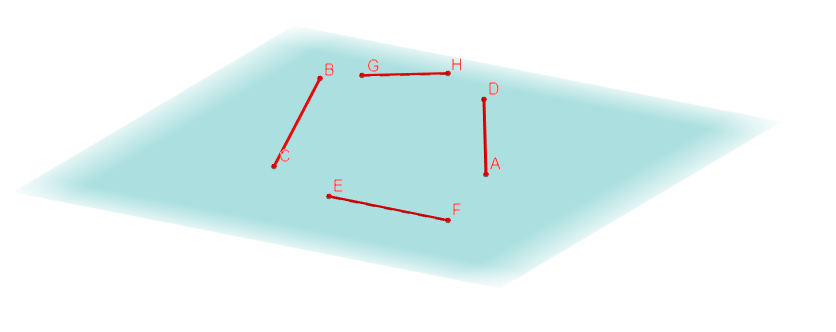
\includegraphics[width=0.7\textwidth]{inoneplane.png}
\end{figure}
Однако такой способ записи довольно громоздкий и, помимо этого, дает "кубические" условия, налагаемые на задачу. С другой стороны можно ввести новые переменные $A_{k},B_{k},C_{k},D_{k}, \forall k=\overline{1,n_{3}}$-коэффициенты из уравнений плоскостей. Они не участвуют в записи минимализируемого функционала, однако с помощью них условия принадлежности одной грани можно записать достаточно просто:
$$
\begin{cases}
A_{k}\tilde{x}_{j,1}+B_{k}\tilde{y}_{j,1}+C_{k}\tilde{z}_{j,1}+D_{k}=0, \forall j \in f_{k} 
\\ 
A_{k}\tilde{x}_{j,2}+B_{k}\tilde{y}_{j,2}+C_{k}\tilde{z}_{j,2}+D_{k}=0, \forall j \in f_{k}
\\
A_{k}^{2}+B_{k}^{2}+C_{k}^{2}=1-\text{ нормировка коэффициентов}
\end{cases}
$$
\begin{wrapfigure}[14]{r}{0.25\linewidth} 

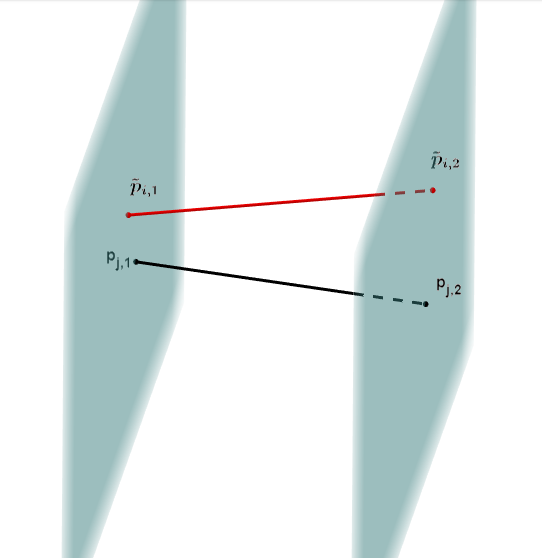
\includegraphics[width=0.4\textwidth]{innormalplane.png}
\end{wrapfigure}
\par
Не менее важными являются условия принадлежности концов "подвижных" ребер нормальным плоскостям изначальных ребер многогранника (нецелевым). Их можно записать следующим образом:
$$
\begin{cases}
\tilde{p}_{j,1} \in N(p_{e_{j}[1]},e_{j})\\
\tilde{p}_{j,2} \in N(p_{e_{j}[2]},e_{j})
\end{cases}
$$
где $N(p,e)$-плоскость, нормальная к вектору $e$ и проходящая через точку $p$.\par
Данные условия нужны для предотвращения разбегания подвижных ребер. 
\section{Построение многогранника по набору полупространств.}
После решения задачи оптимизации мы имеем наборы подвижных ребер и плоскостей, в которых они лежат. Однако нам хотелось бы по этим данным построить многогранник. Решить эту задачу поможет алгоритм, описанный ниже.
\par
Для начала получим из набора плоскостей-полупространства. Для этого вычислим центр масс исходного многогранника и подставим его в уравнения плоскостей, если получаем положительное число, то плоскость задана внутренней нормалью, поэтому умножим коэффициенты плоскости на -1. Теперь мы имеем множество полупространств, пересечением которых является искомый многогранник. 
\par
Перейдем к алгоритму построения многогранника по набору полупространств:
\begin{algorithm}[H]

x=1\;
cub=createCub(x)\;
\While{ True}{
oldFacets=cub.facets\;
\For{plane $\in$ planes}
{
newFacet=$\varnothing$\;
newEdges=$\varnothing$\;
\For{facet $\in$ cub.facets}
{
newPoints=$\varnothing$\;
\For{ edge $\in$ facet.edges}
{
\If{edge $\cap$ plane $\neq \varnothing$}
{
newPoints=newPoints $\cup$ (edge $\cap$ plane)\;
}
reconstructEdge(edge)\;
}
reconstructFacet(facet)\;
newEdges=newEdges $\cup$ edgeConstruct(newPoints)
}
newFacet=facetConstruct(newEdges)\;
cub.facets=cub.facets $\cup$ newFacet\;
}
\eIf{cub.facets $\cap$ oldFacets =$\varnothing$}
{
break\;
}
{
x=2x\;
cub=createCub(x)\;
}
}

\end{algorithm}
\begin{wrapfigure}[15]{r}{0.4\linewidth} 

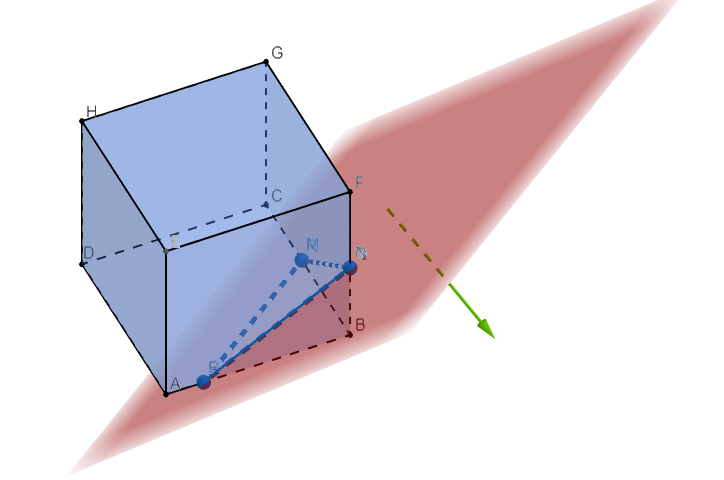
\includegraphics[width=0.6\textwidth]{cub3.png}
\end{wrapfigure}
Изначально мы создаем объемлющий куб, от которого будем отсекать полупространства. Опишем процедуру отсечения плоскости от куба. Мы проходим по всем граням объемлющего куба и в каждой грани смотрим на пересечение всех ребер этой грани с отсекаемой плоскостью. После получения точек пересечения мы изменяем ребра (берем только ту часть ребра, которая лежит в нужном полупространстве) и добавляем к гране ребро пресечения. Ребра, целиком лежащие в противоположном полупространстве-удаляются. Запоминая ребра пересечения мы формируем из них новую грань объемлющего куба (теперь это уже не куб, а объемлющий многогранник) и добавляем ее к его структуре. Проделывая так со всем списком полупространств мы получаем некий многогранник. Однако исходно объемлющий куб мог быть слишком мал, поэтому если после пересечения полупространств в многограннике осталась часть грани исходного объемлющего куба, то мы увеличиваем его размер вдвое и запускаем процесс заново. 
\par
Следует отметить, что алгоритм требует рассмотрения большого числа крайних случаев: пересечение по вершине, ребру, плоскости. 

\section{Средства программной реализации задачи.}
\subsection{IPOPT}
Метод внутренней точки реализован в библиотеке IPOPT. Опишем процесс установки этой библиотеки.
\begin{enumerate} 
\item Скачаем библиотеку из репозитория:
\begin{verbatim}
$ svn co https://projects.coin-or.org/svn/Ipopt/stable/3.12 CoinIpopt 
\end{verbatim}
\item Перейдем в папку с дистрибутивом IPOPT:
\begin{verbatim}
$ cd CoinIpopt
\end{verbatim}
\item Скачаем сторонние библиотеки, необходимые для сборки IPOPT:
\begin{verbatim}
$ cd /ThirdParty/Blas 
$ ./get.Blas 
$ cd ..
$cd Lapack 
$ ./get.Lapack 
$ cd ..
$cd ASL 
$ ./get.ASL
и т.д. для всех папок в ThirdPart
\end{verbatim}
\item Создаём каталог build:
\begin{verbatim}
$ mkdir build 
\end{verbatim}
и переходим в него:
\begin{verbatim}
$ cd build 
\end{verbatim}
\item Запускаем скрипт configure:
\begin{verbatim}
$ ../configure 
\end{verbatim}
\item Собираем:
\begin{verbatim}
$ make
\end{verbatim}
\item Запускаем короткий тест, чтобы проверить, что компиляция прошла успешно:
\begin{verbatim}
$ make test
\end{verbatim}
\item Устанавливаем IPOPT:
\begin{verbatim}
$ make install
\end{verbatim}
После этого в каталоге bin должен появиться исполняемый файл ipopt.
\item Переходим в корневую папку:
\begin{verbatim}
$ cd 
\end{verbatim}
И затем в bin:
\begin{verbatim}
$ cd bin
\end{verbatim}
Сохраняем в эту папку файл ipopt. 
\end{enumerate} 
\subsection{C++ Интерфейс}
Основным классом, с которым предстоит работать является MyNLP, унаследованный от стандартного класса Ipopt::TNLP. В нем должны быть определены следующие методы класса:
\begin{enumerate}
\item 
\begin{verbatim}bool MyNLP::get_nlp_info(Index& n, Index& m, Index& nnz_jac_g,
Index& nnz_h_lag, IndexStyleEnum& index_style)
\end{verbatim}

Задает общую информацию о задаче: число переменных, число ограничений, число ненулевых элементов матрицы Якоби для ограничений, число ненулевых элементов матрицы Гесса для функции Лагранжа.
\item 
\begin{verbatim}
bool MyNLP::get_bounds_info(Index n, Number* x_l, Number* x_u,
Index m, Number* g_l, Number* g_u)
\end{verbatim}

Задает ограничения на переменные и на условия. Если ограничений нет, то
\begin{verbatim} 
x_l[i] = -1.0e19;
x_u[i] = 1.0e19;
\end{verbatim}
\item 
\begin{verbatim}
bool MyNLP::get_starting_point(Index n, bool init_x, Number* x,
bool init_z, Number* z_L, Number* z_U,
Index m, bool init_lambda,
Number* lambda)
\end{verbatim}
Задает стартовую точку алгоритма. Важно, чтобы она удовлетворяла всем условиям g. Алгоритм не просто так называется алгоритмом внутренней точки. 
\item 
\begin{verbatim}
bool MyNLP::eval_f(Index n, const Number* x, bool new_x, Number& obj_value)
\end{verbatim}
Здесь нужно задать минимализируемый функционал. 
\item 
\begin{verbatim}
bool MyNLP::eval_grad_f(Index n, const Number* x, bool new_x, Number* grad_f)
\end{verbatim}
Посчитать градиент от функционала. 
\item
\begin{verbatim}
bool MyNLP::eval_g(Index n, const Number* x, bool new_x, Index m, Number* g)
\end{verbatim}
В этой функции мы задаем ограничения на функционал. 
\item
\begin{verbatim}
bool MyNLP::eval_jac_g(Index n, const Number* x, bool new_x,
Index m, Index nele_jac, Index* iRow, Index *jCol,
Number* values)
\end{verbatim}
Здесь задается структура ненулевых элементов матрицы Якоби. 
\begin{verbatim}
iRow[i]=rowNumber;
jCol[i] = colNumber;
\end{verbatim}
А затем значение этого элемента 
\begin{verbatim}
values[i]=value;
\end{verbatim}
\item
\begin{verbatim}
bool MyNLP::eval_h(Index n, const Number* x, bool new_x,
Number obj_factor, Index m, const Number* lambda,
bool new_lambda, Index nele_hess, Index* iRow,
Index* jCol, Number* values)
\end{verbatim}
Вычисление Гессиана от Лагранжиана функционала. Можно пропустить, написав специальную команду в опциях компиляции. 
\item
\begin{verbatim}
void MyNLP::finalize_solution(SolverReturn status,
Index n, const Number* x, const Number* z_L, const Number* z_U,
Index m, const Number* g, const Number* lambda,
Number obj_value,
const IpoptData* ip_data,
IpoptCalculatedQuantities* ip_cq)
\end{verbatim}
То, что будет выполнено по завершению поиска оптимума. Здесь я запускаю построение многогранника по набору полупространств и его последующую отрисовку.
\end{enumerate}
\section{Результаты работы программной реализации модели.}

\subsection{Первый тестовый многогранник.}
\begin{center}
\begin{tabular}{|c|c|}
\hline
Перестроенный многогранник & Ошибка на ребрах\\
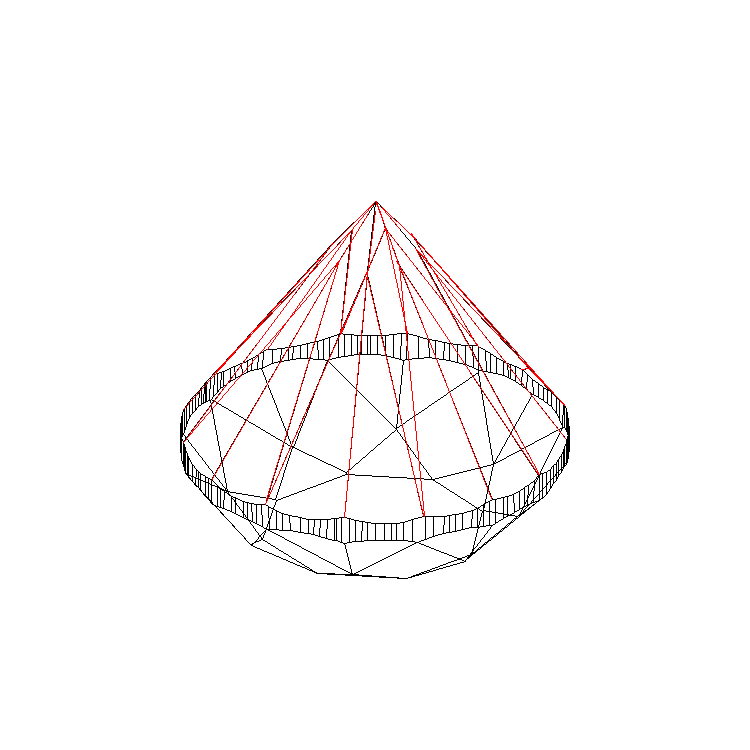
\includegraphics[width=0.5\textwidth]{bigout1.png} &
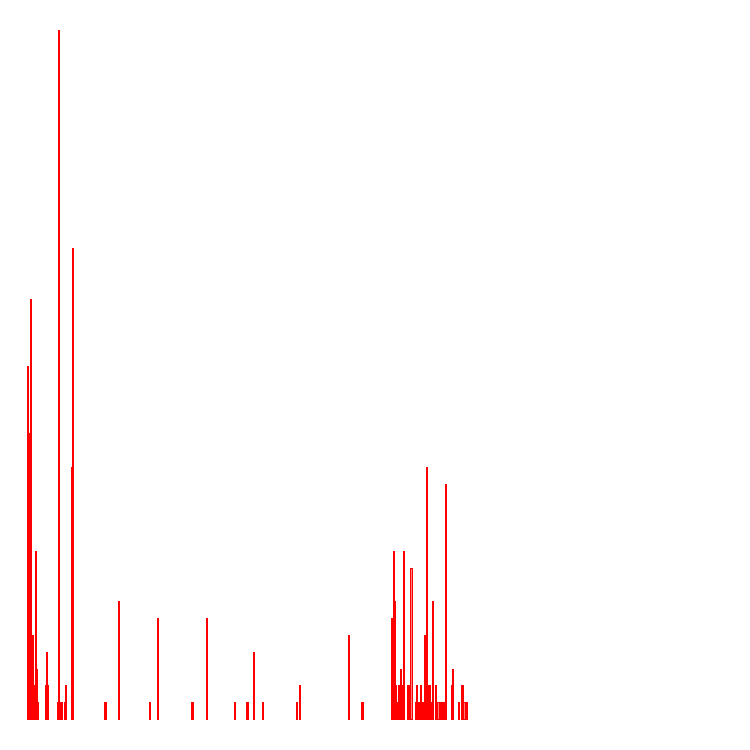
\includegraphics[width=0.5\textwidth]{bigerror1.png} \\ 
\hline
\end{tabular}
\end{center}
\textbf{Значение функционала:} $3.9*10^{-4}$\\
\textbf{Время работы:} $405$ секунд\\
\textbf{Число итераций:} $478$\\
\textbf{Число вершин:} $442$\\
\textbf{Число ребер:} $663$\\
\textbf{Число граней:} $223$\\
\textbf{Число целевых ребер:} $35$ \\
\textbf{Число переменных:} $4870$\\
\textbf{Число ненулевых элементов в Якобиане:} $9951$\\
\newpage
\subsection{Второй тестовый многогранник.}
\begin{center}
\begin{tabular}{|c|c|}
\hline
Перестроенный многогранник & Ошибка на ребрах\\
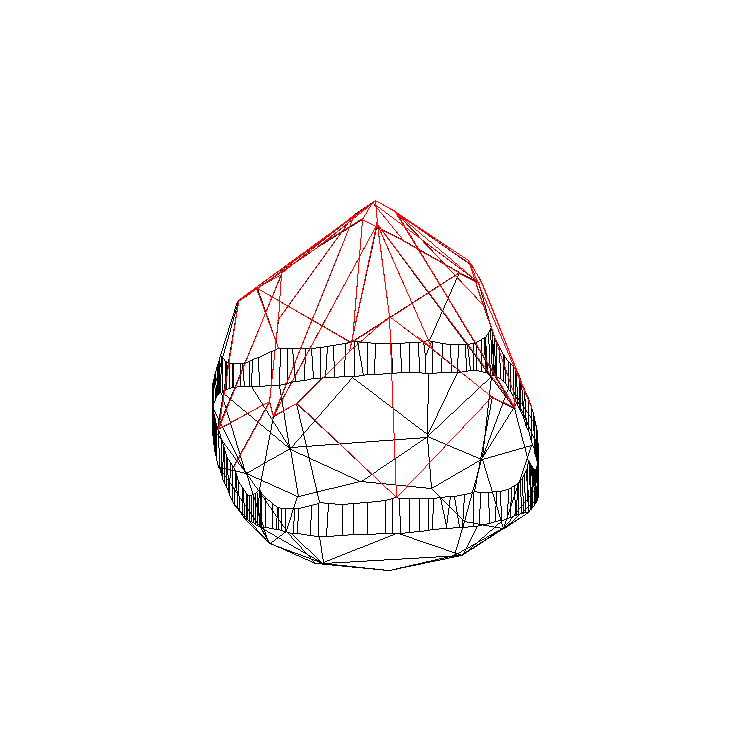
\includegraphics[width=0.5\textwidth]{bigout2.png} &
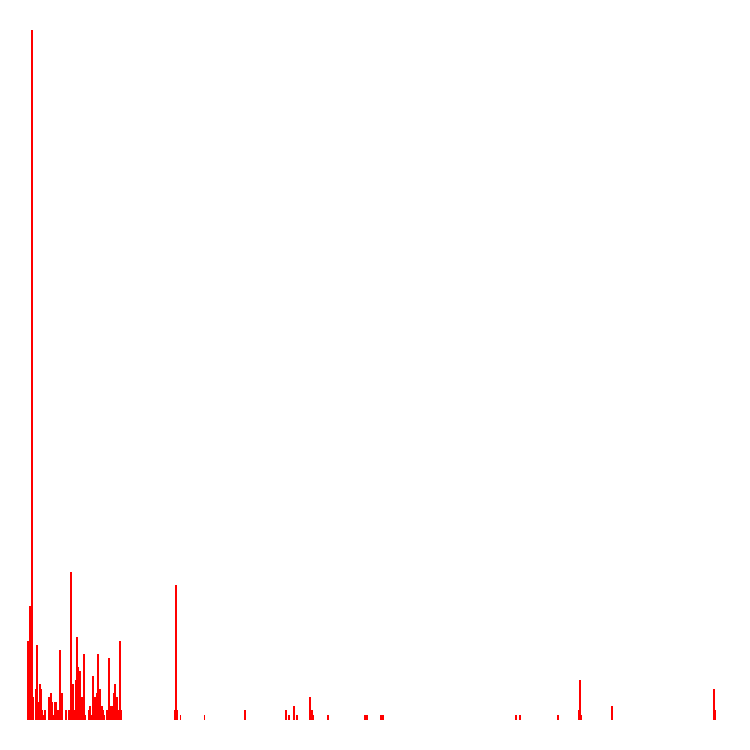
\includegraphics[width=0.5\textwidth]{bigerror2.png} \\ 
\hline
\end{tabular}
\end{center}
\textbf{Значение функционала:} $7.6*10^{-4}$\\
\textbf{Время работы:} $635$ секунд\\
\textbf{Число итераций:} $526$\\
\textbf{Число вершин:} $536$\\
\textbf{Число ребер:} $804$\\
\textbf{Число граней:} $270$\\
\textbf{Число целевых ребер:} $68$ \\
\textbf{Число переменных:} $5904$\\
\textbf{Число ненулевых элементов в Якобиане:} $12066$\\
\section{Ускорение работы на больших моделях.}
К сожалению, на больших моделях алгоритм работает долго. Однако из гистограмм ошибок можно заметить, что на более чем половине ребер удаление от целевых ребер-нулевое. Это ребра нижней части кристалла, для которых изначально нет целевых ребер и они притягиваются сами к себе. В результате этого они являются статичными и их движения не происходит, однако обсчет их движения происходит. Будем теперь включать в функционал только ребра, лежащие в гранях, в которые входит хотя бы одно целевое ребро. Такая модель несколько сложнее программируется, но, даст ускорение в десятки раз.  Так первый кристалл приближается за 10 секунд после 37 итераций, а второй-за 20 секунд после 41 итерации.
\section{Сведение задачи к задаче безусловной оптимизации}
Будем теперь считать неизвестными уравнения плоскостей, в которых лежат грани кристалла. Для дальнейших рассуждений введем следующие обозначения:
$$
\begin{cases}
e_{i} = (p_{i}^{0}, p_{i}^{1}) \text{ - ребра многогранника} \\
\widetilde{e_{i}} =(\widetilde{p_{i}^{0}}, \widetilde{ p_{i}^{1}}) \text{ - соотвествующие целевые ребра} \\
\begin{rcases}
\Pi_{i}^{0}: A_{i}^{0}x+B_{i}^{0}y+C_{i}^{0}z+D_{i}^{0}=0\\
\Pi_{i}^{1}: A_{i}^{1}x+B_{i}^{1}y+C_{i}^{1}z+D_{i}^{1}=0\\
\end{rcases} \Pi_{i}^{0} \cap \Pi_{i}^{1}=e_{i} \\
N_{i}^{0}: a_{i}^{0}x+b_{i}^{0}y+c_{i}^{0}z+d_{i}^{0}=0 : N_{i}^{0} \perp e_{i}, p_{i}^{0} \in N_{i}^{0} \\
N_{i}^{1}: a_{i}^{1}x+b_{i}^{1}y+c_{i}^{1}z+d_{i}^{1}=0: N_{i}^{1} \perp e_{i}, p_{i}^{1} \in N_{i}^{1} \\
\end{cases}
$$ 
Из этих обозначений напряую следует, что вершины ребер $$p_{i}^{0}=(x_{i}^{0}, y_{i}^{0}, z_{i}^{0}) $$ $$ p_{i}^{1}=(x_{i}^{1}, y_{i}^{1}, z_{i}^{1})$$ являются соответственно решениями систем:

\begin{equation}
\label{eq1}
\begin{cases}
A_{i}^{0}x_{i}^{0}+B_{i}^{0}y_{i}^{0}+C_{i}^{0}z_{i}^{0}+D_{i}^{0}=0\\
A_{i}^{1}x_{i}^{0}+B_{i}^{1}y_{i}^{0}+C_{i}^{1}z_{i}^{0}+D_{i}^{1}=0\\
a_{i}^{0}x_{i}^{0}+b_{i}^{0}y_{i}^{0}+c_{i}^{0}z_{i}^{0}+d_{i}^{0}=0 
\end{cases} 
\end{equation}

\begin{equation}
\label{eq2}
\begin{cases}
A_{i}^{0}x_{i}^{1}+B_{i}^{0}y_{i}^{1}+C_{i}^{0}z_{i}^{1}+D_{i}^{0}=0\\
A_{i}^{1}x_{i}^{1}+B_{i}^{1}y_{i}^{1}+C_{i}^{1}z_{i}^{1}+D_{i}^{1}=0\\
a_{i}^{1}x_{i}^{1}+b_{i}^{1}y_{i}^{1}+c_{i}^{1}z_{i}^{1}+d_{i}^{1}=0 
\end{cases} 
\end{equation}
Откуда следуют зависимости:
$$
x_{i}^{0} = x_{i}^{0}(A_{i}^{0}, B_{i}^{0}, C_{i}^{0}, D_{i}^{0}, A_{i}^{1}, B_{i}^{1}, C_{i}^{1}, D_{i}^{1}) 
$$
$$
y_{i}^{0} = y_{i}^{0}(A_{i}^{0}, B_{i}^{0}, C_{i}^{0}, D_{i}^{0}, A_{i}^{1}, B_{i}^{1}, C_{i}^{1}, D_{i}^{1}) 
$$
$$
z_{i}^{0} = z_{i}^{0}(A_{i}^{0}, B_{i}^{0}, C_{i}^{0}, D_{i}^{0}, A_{i}^{1}, B_{i}^{1}, C_{i}^{1}, D_{i}^{1}) 
$$
$$
x_{i}^{1} = x_{i}^{1}(A_{i}^{0}, B_{i}^{0}, C_{i}^{0}, D_{i}^{0}, A_{i}^{1}, B_{i}^{1}, C_{i}^{1}, D_{i}^{1}) 
$$
$$
y_{i}^{1} = y_{i}^{1}(A_{i}^{0}, B_{i}^{0}, C_{i}^{0}, D_{i}^{0}, A_{i}^{1}, B_{i}^{1}, C_{i}^{1}, D_{i}^{1}) 
$$
$$
z_{i}^{1} = z_{i}^{1}(A_{i}^{0}, B_{i}^{0}, C_{i}^{0}, D_{i}^{0}, A_{i}^{1}, B_{i}^{1}, C_{i}^{1}, D_{i}^{1})
$$ 
Введем теперь функционал, который будем минимализировать:

\begin{multline}
\Phi = \sum \limits_{i=0}^{n} \rho^{2}(\widetilde{p_{i}^{0}},p_{i}^{0}(A_{i}^{0}, B_{i}^{0}, C_{i}^{0}, D_{i}^{0}, A_{i}^{1}, B_{i}^{1}, C_{i}^{1}, D_{i}^{1}))+ \\
\rho^{2}(\widetilde{p_{i}^{1}},p_{i}^{1}(A_{i}^{0}, B_{i}^{0}, C_{i}^{0}, D_{i}^{0}, A_{i}^{1}, B_{i}^{1}, C_{i}^{1}, D_{i}^{1}))
\rightarrow \min
\end{multline}

\begin{multline}
\Phi = \sum \limits_{i=0}^{n} 
(\widetilde{x_{i}^{0}}-x_{i}^{0})^{2}+
(\widetilde{y_{i}^{0}}-y_{i}^{0})^{2}+
(\widetilde{z_{i}^{0}}-z_{i}^{0})^{2}+\\
(\widetilde{x_{i}^{1}}-x_{i}^{1})^{2}+
(\widetilde{y_{i}^{1}}-y_{i}^{1})^{2}+
(\widetilde{z_{i}^{1}}-z_{i}^{1})^{2} \rightarrow \min
\end{multline}


Осуществять поиск минимума будем методом градиентного спуска. Соответсвенно необходимо уметь считать градиент: $\nabla \Phi = (\frac{\partial \Phi}{\partial A_{0}^{0}}, \hdots, \frac{\partial \Phi}{\partial D_{n}^{1}})$ \\
Для примера рассмотрим компоненту градиента, вычисленую по формуле сложной функции 

$$
\begin{matrix}
\frac{\partial \Phi}{\partial A_{i}^{0}}=-2(\widetilde{x_{i}^{0}}-x_{i}^{0})\frac{\partial x_{i}^{0}}{\partial A_{i}^{0}}-2(\widetilde{y_{i}^{0}}-y_{i}^{0})\frac{\partial y_{i}^{0}}{\partial A_{i}^{0}}-2(\widetilde{z_{i}^{0}}-z_{i}^{0})\frac{\partial z_{i}^{0}}{\partial A_{i}^{0}}\\
-2(\widetilde{x_{i}^{1}}-x_{i}^{1})\frac{\partial x_{i}^{1}}{\partial A_{i}^{0}}-2(\widetilde{y_{i}^{1}}-y_{i}^{1})\frac{\partial y_{i}^{1}}{\partial A_{i}^{0}}-2(\widetilde{z_{i}^{1}}-z_{i}^{1})\frac{\partial z_{i}^{1}}{\partial A_{i}^{0}}
\end{matrix}
$$
Остальные компоненты градиента имеют аналогичный вид. Отсюда следует, что для вычисления градиента $\nabla \Phi$ достаточно знать значения координат вершин $x_{i}^{0}, \hdots , z_{i}^{1}$ и их градиенты $\nabla x_{i}^{0}, \hdots, \nabla  z_{i}^{1}$. Если для получения значений координат вершин достаточно решить системы \ref{eq1} и  \ref{eq2}, то для нахождения градиентов эти системы необходимо продифференцировать по $A_{i}^{0},\hdots, D_{i}^{1}$, а затем решить относительно частных производных. Так, если продифференцировать \ref{eq1} по $A_{i}^{0}$, то получим:
$$
\begin{cases}
x_{i}^{0}+A_{i}^{0}\frac{\partial x_{i}^{0}}{\partial A_{i}^{0}}+B_{i}^{0}\frac{\partial y_{i}^{0}}{\partial A_{i}^{0}}+C_{i}^{0}\frac{\partial z_{i}^{0}}{\partial A_{i}^{0}}=0\\
A_{i}^{1}\frac{\partial x_{i}^{0}}{\partial A_{i}^{0}}+B_{i}^{1}\frac{\partial y_{i}^{0}}{\partial A_{i}^{0}}+C_{i}^{1}\frac{\partial z_{i}^{0}}{\partial A_{i}^{0}}=0\\
a_{i}^{0}\frac{\partial x_{i}^{0}}{\partial A_{i}^{0}}+b_{i}^{0}\frac{\partial y_{i}^{0}}{\partial A_{i}^{0}}+c_{i}^{0}\frac{\partial z_{i}^{0}}{\partial A_{i}^{0}}=0
\end{cases} 
\Leftrightarrow
\begin{cases}
A_{i}^{0}\frac{\partial x_{i}^{0}}{\partial A_{i}^{0}}+B_{i}^{0}\frac{\partial y_{i}^{0}}{\partial A_{i}^{0}}+C_{i}^{0}\frac{\partial z_{i}^{0}}{\partial A_{i}^{0}}=-x_{i}^{0}\\
A_{i}^{1}\frac{\partial x_{i}^{0}}{\partial A_{i}^{0}}+B_{i}^{1}\frac{\partial y_{i}^{0}}{\partial A_{i}^{0}}+C_{i}^{1}\frac{\partial z_{i}^{0}}{\partial A_{i}^{0}}=0\\
a_{i}^{0}\frac{\partial x_{i}^{0}}{\partial A_{i}^{0}}+b_{i}^{0}\frac{\partial y_{i}^{0}}{\partial A_{i}^{0}}+c_{i}^{0}\frac{\partial z_{i}^{0}}{\partial A_{i}^{0}}=0
\end{cases} 
$$
$$
\begin{pmatrix}
A_{i}^{0} & B_{i}^{0} & C_{i}^{0} \\
A_{i}^{1} & B_{i}^{1} & C_{i}^{1} \\
a_{i}^{0} & b_{i}^{0} & c_{i}^{0} 
\end{pmatrix}
\begin{pmatrix}
\frac{\partial x_{i}^{0}}{\partial A_{i}^{0}} \\
\frac{\partial y_{i}^{0}}{\partial A_{i}^{0}} \\
\frac{\partial z_{i}^{0}}{\partial A_{i}^{0}}
\end{pmatrix}
=
\begin{pmatrix}
-x_{i}^{0}\\
0\\
0\\
\end{pmatrix}
$$
Решив систему получим $(\frac{\partial x_{i}^{0}}{\partial A_{i}^{0}}, \frac{\partial y_{i}^{0}}{\partial A_{i}^{0}},\frac{\partial z_{i}^{0}}{\partial A_{i}^{0}})$. Решив остальные системы получим все значения $\nabla x_{i}^{0}, \hdots, \nabla  z_{i}^{1}$, а следоательно и $\nabla \Phi$. Теперь можно применять градиентный спуск. 
\newpage
\begin{thebibliography}{5}
\bibitem{1}
Веселов А. П., Троицкий Е. В. Лекции по аналитической геометрии. Учебное пособие. –– Изд. новое. –– М.: МЦНМО, 2016. –– 152 с. 
\bibitem{2}
Алексеев В.М., Галеев Э.М., Тихомиров В.М. Сборник задач по оптимизации. Теория. Примеры. Задачи: Учеб. пособие. --- 2-е изд. М.: ФИЗМАТЛИТ, 2005. --- 256 с.
\bibitem{3}
О.А. Щербина КРАТКОЕ ВВЕДЕНИЕ В AMPL - CОВРЕМЕННЫЙ АЛГЕБРАИЧЕСКИЙ ЯЗЫК МОДЕЛИРОВАНИЯ (препринт), 2012. --- 29 c. 
\bibitem{4}
Попов А.В. GNUPLOT и его приложения. --- М.: Издательство попечительского совета механико-математического факультета МГУ, 2015 , ---240 с. 
\bibitem{5} Introduction to Ipopt: A tutorial for downloading, installing, and using Ipopt. July 20, 2016
\end{thebibliography}
\end{document}
